\begin{Figure}

    \HEADING{Rdesigneur makes multiscale modeling easier}

    \TEXT{Rdesigneur (\textbf{R}eaction-\textbf{D}iffusion and
        \textbf{E}lectrical \textbf{SIG}naling in \textbf{NEUR}on) makes it
        easier to mix models across scales}
        
    \begin{itemize}
        \item \TEXT{Neuron morphology and network, \texttt{NeuroMorpho,
                    NeuroML}}
        \item \TEXT{Chemical pathways, Reaction diffusion models, \texttt{System
                Biology Markup Language (SBML, DOQCS, KKIT)}}

        \item \TEXT{Ion-channels models \texttt{channelpedia, OpenSourceBrain}}
    \end{itemize}
    
    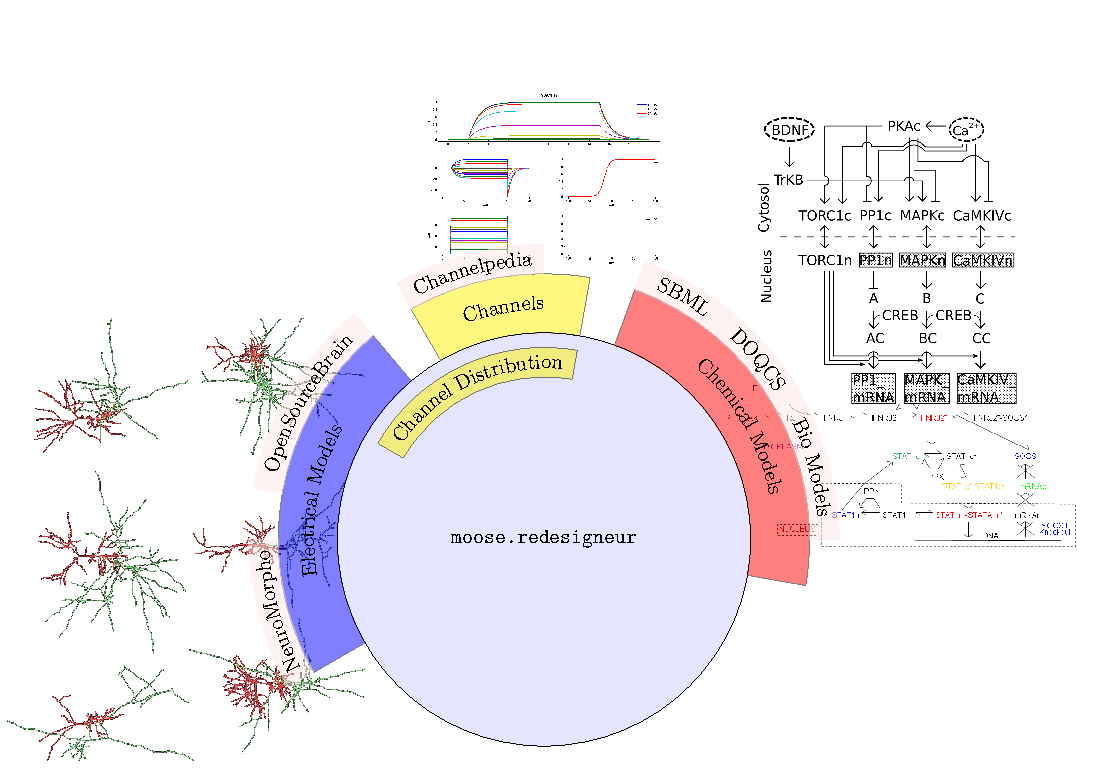
\includegraphics[width=\textwidth]{./_images/rdesigneur.pdf}

    \vspace{2cm}
    \HEADING{Supported Platforms}

    \TEXT{All major Linux flavors}
    \includegraphics[width=\textwidth]{./_images/supported_platforms.png}
    \TEXT{Cygwin/Windows, MacOSX, Supports GCC/LLVM compilers}
    \includegraphics[width=\textwidth]{./_images/supported_platforms1.png}

    \vspace{1cm}
    \HEADING{Summary}

    \raggedright

    \TEXT{\bf We use models to:}
    \begin{itemize}

        \item \TEXT{Integrate many scales of neuronal data with basic
            physical/chemical principles.}
        \item \TEXT{Explain phenomena of plasticity, activity and neuronal
                coding.}
        \item \TEXT{Predict circuit mechanisms, plasticity rules, and emergent
            phenomena such as {decorrelation}, {robustness}, and
            {memory decay}.}

    \end{itemize}

 
\end{Figure}


